% !TeX program = pdflatex
% Apresentação de qualificação — Fernando Souza da Vieira
% Estrutura: título + 12 slides de conteúdo + agradecimentos.
% Compilar nesta pasta para que os caminhos em assets/ sejam encontrados.

\documentclass[aspectratio=169,11pt]{beamer}

% Pacotes usuais em apresentações acadêmicas em LaTeX.
\usepackage[T1]{fontenc}
\usepackage[utf8]{inputenc}
\usepackage{lmodern}
\usepackage{amsmath,amssymb}
\usepackage{booktabs,array}
\usepackage{graphicx}

% Tema canônico do Beamer, sem identidade visual customizada.
\usetheme{Boadilla}
\usecolortheme{default}
\usefonttheme{serif}
\setbeamertemplate{navigation symbols}{}
\setbeamertemplate{caption}[numbered]
\setbeameroption{hide notes}

\title[Comensalismo Econômico]{Comensalismo Econômico}
\subtitle{Governando os comuns por incentivos racionais}
\author[F. S. Vieira]{Fernando Souza da Vieira}
\institute[FEARP/USP]{FEARP/USP\\Orientador: Prof. Dr. Alexandre Chibebe Nicolella}
\date{Qualificação do projeto de doutorado}

\begin{document}

% -----------------------------------------------------------------------------
% TÍTULO — não conta entre os 12 slides de conteúdo.
% GUIA: apresentar o tema como uma pergunta de economia, não como uma analogia
% biológica já resolvida.
% -----------------------------------------------------------------------------
\begin{frame}[plain,noframenumbering]
  \titlepage
  \note{
    Abrir pela tensão entre decisão privada e preservação. O termo
    ``comensalismo'' será tratado como hipótese de uma relação econômica nova,
    cuja coerência ainda precisa ser demonstrada.
  }
\end{frame}

% -----------------------------------------------------------------------------
% 1. PONTO DE PARTIDA
% GUIA: deixar claro que o conflito é econômico e intertemporal.
% -----------------------------------------------------------------------------
\begin{frame}{1. Produção e preservação}
  \begin{itemize}
    \item Produção gera renda, emprego e bem-estar.
    \item Degradação compromete a base ecológica da produção futura.
    \item Para o agente privado, preservar pode aparecer como custo imediato.
  \end{itemize}

  \vfill
  \begin{block}{Problema}
    Tornar a preservação compatível com produtividade e rentabilidade privadas.
  \end{block}

  \note{
    Não apresentar produção e preservação como escolhas morais opostas. O ponto
    econômico é a diferença entre benefícios privados imediatos e benefícios
    ecológicos frequentemente tardios, incertos e difusos.
  }
\end{frame}

% -----------------------------------------------------------------------------
% 2. LACUNA
% GUIA: evitar a afirmação forte de que a economia ``ignora'' a natureza.
% -----------------------------------------------------------------------------
\begin{frame}{2. Onde está a lacuna?}
  \begin{block}{A teoria econômica não ignora a natureza}
    Recursos naturais, externalidades, bens comuns e capital natural já são
    objetos centrais da literatura.
  \end{block}

  \vspace{0.4cm}
  \begin{itemize}
    \item O ambiente aparece como insumo, estoque, restrição ou externalidade.
    \item Falta integrar, no mesmo problema:
      \begin{itemize}
        \item funcionalidade ecológica;
        \item produção e retornos privados;
        \item governança na escala territorial relevante.
      \end{itemize}
  \end{itemize}

  \note{
    Esta formulação segue o Artigo 1 atual. A contribuição pretendida não é
    ``introduzir a natureza na economia'', mas integrar elementos que aparecem
    separados e explicitar as condições em que a preservação entra na decisão
    privada.
  }
\end{frame}

% -----------------------------------------------------------------------------
% 3. PERGUNTA E OBJETIVO
% GUIA: ler a pergunta e, depois, traduzi-la em um objetivo operacional.
% -----------------------------------------------------------------------------
\begin{frame}{3. Pergunta de pesquisa}
  \begin{block}{Pergunta}
    É possível conciliar, de forma efetiva e eficiente, produtividade e
    rentabilidade privadas com preservação ambiental socialmente desejável,
    mediante incentivos bem estruturados, superando o desempenho do sistema
    extrativista atual?
  \end{block}

  \vspace{0.35cm}
  \begin{block}{Objetivo geral}
    Investigar um arranjo econômico-institucional que permita otimizar
    conjuntamente resultados econômicos e ecológicos.
  \end{block}

  \note{
    A pergunta é deliberadamente ambiciosa. A tese não parte da resposta
    afirmativa como fato. Cada artigo verifica uma dimensão necessária dessa
    resposta: coerência teórica, estabilidade e evidência empírica.
  }
\end{frame}

% -----------------------------------------------------------------------------
% 4. HIPÓTESES
% GUIA: preservar a estrutura H1--H5 do pré-projeto.
% -----------------------------------------------------------------------------
\begin{frame}{4. Hipóteses que organizam a tese}
  \small
  \begin{description}
    \item[H1] A funcionalidade ambiental deve ser endogenizada na produção.
    \item[H2] A decisão é intertemporal, sob incerteza e racionalidade limitada.
    \item[H3] Incentivos devem respeitar escalas territoriais e ecológicas.
    \item[H4] Incentivos calibrados podem tornar a preservação racional.
    \item[H5] A interação pode convergir para um equilíbrio estratégico estável.
  \end{description}

  \vfill
  \centering
  \textbf{H0:} é possível um arranjo compatível com incentivos que alinhe
  desempenho privado e ambiental.

  \note{
    As cinco hipóteses não são cinco teses independentes. H1 estabelece a
    representação; H2 e H3 introduzem tempo e espaço; H4 trata do mecanismo de
    incentivo; H5 trata do resultado de equilíbrio.
  }
\end{frame}

% -----------------------------------------------------------------------------
% 5. CONCEITO
% GUIA: usar o gráfico do próprio projeto como intuição, não como prova.
% -----------------------------------------------------------------------------
\begin{frame}{5. O que chamo de comensalismo econômico?}
  \small
  \begin{columns}[T,onlytextwidth]
    \column{0.62\textwidth}
      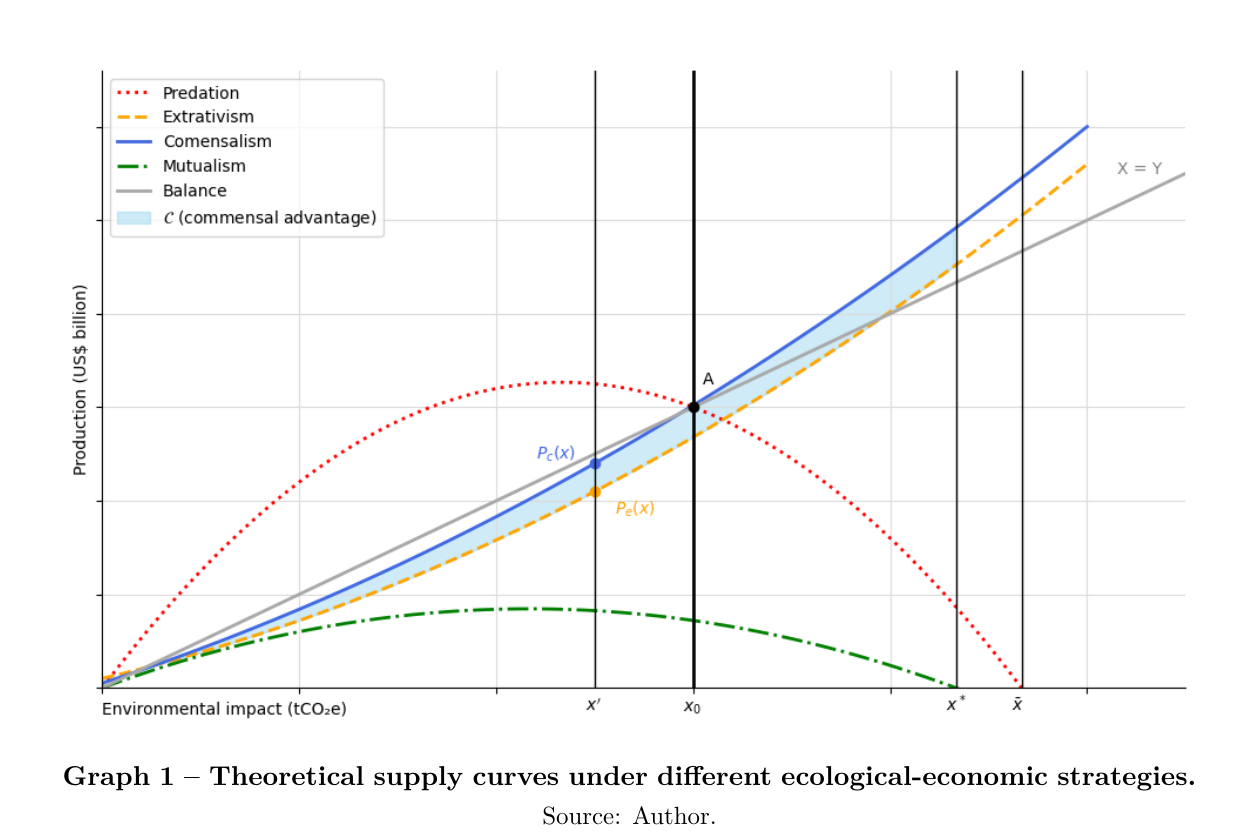
\includegraphics[width=\linewidth]{assets/grafico_estrategias_projeto.png}

    \column{0.34\textwidth}
      \begin{itemize}
        \item \textbf{Neutralidade racional} no uso de recursos naturais.
        \item Preservação compatível com viabilidade privada.
        \item Comparação com predação, extrativismo e mutualismo.
      \end{itemize}

      \begin{alertblock}{Hipótese, não resultado}
        A curva ainda será formalizada e testada.
      \end{alertblock}
  \end{columns}

  \note{
    Explicar o gráfico sem tratá-lo como resultado. Ele organiza quatro relações
    econômico-ecológicas propostas no pré-projeto. O Artigo 1 precisa transformar
    essa intuição em definições, hipóteses e condições comparáveis.

    Fonte da figura: elaboração do autor no pré-projeto.
  }
\end{frame}

% -----------------------------------------------------------------------------
% 6. ARQUITETURA
% GUIA: esta é a resposta mais curta para ``o que cada artigo entrega?''.
% -----------------------------------------------------------------------------
\begin{frame}{6. Três artigos, uma tese}
  \centering
  \small
  \begin{tabular}{>{\bfseries}p{1.8cm}p{5.0cm}p{4.0cm}}
    \toprule
    & Pergunta & Entrega \tabularnewline
    \midrule
    Artigo 1 & A relação pode existir de modo teoricamente coerente? &
      Existência teórica / coerência interna \tabularnewline[0.25cm]
    Artigo 2 & Essa relação permanece estável no tempo? &
      Estabilidade dinâmica \tabularnewline[0.25cm]
    Artigo 3 & Essa relação pode ser observada em Mato Grosso? &
      Existência empírica / coerência externa \tabularnewline
    \bottomrule
  \end{tabular}

  \vfill
  \textbf{Sequência:} conceito $\longrightarrow$ estabilidade $\longrightarrow$ evidência

  \note{
    Esta sequência delimita a tese. O Artigo 1 não precisa demonstrar estabilidade
    nem causalidade empírica. O Artigo 2 não substitui o teste externo. O Artigo 3
    não cria o conceito; confronta suas implicações com casos observáveis.
  }
\end{frame}

% -----------------------------------------------------------------------------
% 7. ARTIGO 1
% GUIA: ser transparente sobre o que já existe e o que ainda falta.
% -----------------------------------------------------------------------------
\begin{frame}{7. Artigo 1 — existência teórica}
  \begin{columns}[T,onlytextwidth]
    \column{0.54\textwidth}
      \begin{itemize}
        \item $E$: funcionalidade ecológica como estado endógeno.
        \item Produção, preservação e instituições afetam $E$.
        \item $E$ afeta produção e retorno privado.
        \item A governança acompanha a escala ecológica relevante.
      \end{itemize}

    \column{0.42\textwidth}
      \begin{block}{Representação inicial}
        \[
          Y=F(K,L,E)
        \]
        \[
          \begin{aligned}
            F_E&>0, & F_{EE}&<0,\\
            F_{KE}&>0, & F_{LE}&>0.
          \end{aligned}
        \]
      \end{block}
  \end{columns}

  \vfill
  \begin{alertblock}{Estado do artigo}
    Introdução estruturada; modelo, resultados e discussão ainda em construção.
  \end{alertblock}

  \note{
    O Artigo 1 atual já reformula corretamente a lacuna como integração analítica.
    Seu núcleo será distinguir recurso natural como insumo de funcionalidade
    ecológica como estado, ligar esse estado aos payoffs e definir condições para
    uma configuração comensal. Não afirmar que as derivadas já foram demonstradas:
    elas são relações esperadas do pré-projeto.
  }
\end{frame}

% -----------------------------------------------------------------------------
% 8. ARTIGO 2
% GUIA: apresentar um núcleo formal e manter os demais instrumentos condicionais.
% -----------------------------------------------------------------------------
\begin{frame}{8. Artigo 2 — estabilidade no tempo}
  \begin{block}{Núcleo planejado}
    Decisão intertemporal + transição ecológica + interação estratégica.
  \end{block}

  \begin{columns}[T,onlytextwidth]
    \column{0.52\textwidth}
      \begin{itemize}
        \item Bellman: escolha entre explorar e preservar.
        \item Markov: choques e transições ambientais.
        \item Aprendizado e racionalidade limitada.
        \item Convergência, limiares e robustez do equilíbrio.
      \end{itemize}

    \column{0.44\textwidth}
      \begin{block}{Extensões previstas}
        Inferência bayesiana, redes de interação, filtro de Kalman e ponto fixo
        de Kakutani.
      \end{block}
      \vspace{0.2cm}
      Cada extensão entra apenas se responder a uma necessidade específica do
      modelo.
  \end{columns}

  \note{
    O pré-projeto contém uma caixa de ferramentas ampla. A estratégia de defesa
    é manter essas possibilidades, mas hierarquizá-las. O modelo mínimo deve ser
    suficiente para definir estado, controle, transição e critério de estabilidade;
    as extensões dependem da pergunta que permanecer aberta.
  }
\end{frame}

% -----------------------------------------------------------------------------
% 9. ARTIGO 3
% GUIA: justificar Mato Grosso pela variação econômica, ecológica e institucional.
% -----------------------------------------------------------------------------
\begin{frame}{9. Artigo 3 — existência empírica}
  \begin{columns}[T,onlytextwidth]
    \column{0.62\textwidth}
      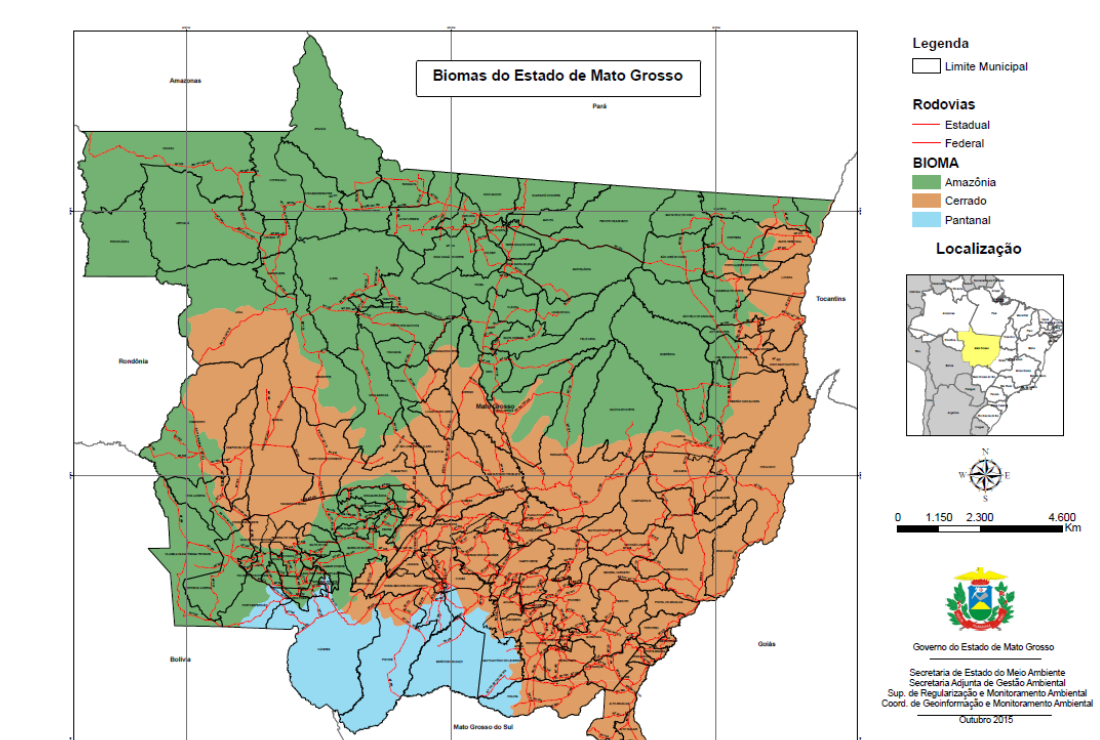
\includegraphics[width=\linewidth]{assets/mapa_biomas_mt.png}

    \column{0.34\textwidth}
      \begin{block}{Por que Mato Grosso?}
        \begin{itemize}
          \item fronteira produtiva;
          \item Amazônia, Cerrado e Pantanal;
          \item incentivos e governança heterogêneos.
        \end{itemize}
      \end{block}

      \begin{block}{Teste externo}
        Há situações com ganho privado sem piora ambiental?
      \end{block}
  \end{columns}

  \note{
    Mato Grosso não é apenas um local de aplicação. A coexistência de três biomas,
    forte produção agropecuária e diferentes arranjos institucionais cria variação
    útil para confrontar as implicações do modelo.

    Fonte do mapa: SEMA-MT, mapa de biomas do Estado de Mato Grosso.
  }
\end{frame}

% -----------------------------------------------------------------------------
% 10. CASOS
% GUIA: tratar a lista como funil de seleção, conforme o próprio pré-projeto.
% -----------------------------------------------------------------------------
\begin{frame}{10. Casos candidatos em Mato Grosso}
  \small
  \begin{tabular}{p{4.1cm}p{7.3cm}}
    \toprule
    Caso & Pergunta possível \tabularnewline
    \midrule
    REM-MT / REDD+ & A remuneração por resultados altera desmatamento e desempenho
      econômico local? \tabularnewline[0.18cm]
    PCI e Carbono Neutro MT & A coordenação territorial produz trajetórias econômicas
      e ambientais distintas? \tabularnewline[0.18cm]
    Mercados de carbono & A participação voluntária muda uso da terra, risco ou
      produtividade? \tabularnewline[0.18cm]
    CAR / CRA e crédito rural & Regularização e incentivos financeiros afetam a
      decisão de preservar? \tabularnewline
    \bottomrule
  \end{tabular}

  \vfill
  \centering
  A seleção final depende de \textbf{dados}, \textbf{tratamento} e
  \textbf{contrafactual defensável}.

  \note{
    Estes casos vêm do pré-projeto, com CAR e crédito como alternativas próximas.
    Não prometer avaliar todos. A escolha deve ocorrer depois de verificar acesso,
    granularidade, período e regra de elegibilidade de cada programa.
  }
\end{frame}

% -----------------------------------------------------------------------------
% 11. DADOS E MODELOS
% GUIA: o desenho de identificação vem antes do estimador.
% -----------------------------------------------------------------------------
\begin{frame}{11. Dados e estratégia empírica}
  \begin{columns}[T,onlytextwidth]
    \column{0.44\textwidth}
      \begin{block}{Dados possíveis}
        \begin{itemize}
          \item INPE / PRODES / DETER;
          \item MapBiomas;
          \item IBGE / PAM / PPM / PIB;
          \item SEMA / SICAR;
          \item crédito rural / SICOR.
        \end{itemize}
      \end{block}

    \column{0.52\textwidth}
      \begin{block}{Modelos possíveis}
        \begin{itemize}
          \item painel com efeitos fixos;
          \item diferenças-em-diferenças / estudo de evento;
          \item controle sintético;
          \item SAR / SDM para efeitos espaciais;
          \item PSM e GWR como apoio ou diagnóstico.
        \end{itemize}
      \end{block}
  \end{columns}

  \vfill
  \centering
  O tratamento e o contrafactual definem o modelo — não o contrário.

  \note{
    Sugestão de sequência: primeiro construir o painel municipal ou por imóvel;
    depois identificar qual programa oferece variação plausivelmente exógena;
    então escolher o estimador. DiD exige tendências paralelas; controle sintético,
    unidade tratada bem definida; SAR/SDM, justificativa para a matriz espacial.
  }
\end{frame}

% -----------------------------------------------------------------------------
% 12. FRAGILIDADES
% GUIA: reconhecer limites como tarefas de pesquisa, sem pedir desculpas pelo projeto.
% -----------------------------------------------------------------------------
\begin{frame}{12. Fragilidades e como serão enfrentadas}
  \small
  \begin{itemize}
    \item \textbf{Novidade.} Posicionar a contribuição frente a capital natural e
      Dasgupta.
    \item \textbf{Formalização.} Definições, hipóteses, proposições e
      contraexemplos no Artigo 1.
    \item \textbf{Escopo dinâmico.} Modelo mínimo; extensões condicionais no
      Artigo 2.
    \item \textbf{Identificação.} Dados, tratamento e contrafactual antes da
      estimação no Artigo 3.
    \item \textbf{Espaço.} Governança entre escalas e testes de transbordamentos.
  \end{itemize}

  \vfill
  \centering
  A ambição permanece; as conclusões serão condicionais às hipóteses e à evidência.

  \note{
    Encerrar mostrando controle sobre os riscos do projeto. A principal defesa não
    é negar as fragilidades, mas atribuir a cada artigo uma tarefa verificável. A
    novidade deve ser demonstrada frente à literatura, não apenas declarada.
  }
\end{frame}

% -----------------------------------------------------------------------------
% AGRADECIMENTOS — não conta entre os 12 slides de conteúdo.
% GUIA: deixar a pergunta central disponível para iniciar o debate.
% -----------------------------------------------------------------------------
\begin{frame}[plain,noframenumbering]
  \centering
  \vfill
  {\LARGE Obrigado.}

  \vspace{0.8cm}
  {\large Comentários e críticas são bem-vindos.}
  \vfill

  \note{
    Retomar, se necessário: a tese investiga existência teórica, estabilidade e
    existência empírica de uma relação econômico-ecológica comensal.
  }
\end{frame}

\end{document}
